\chapter{The Optical Flow Equation}
\sectionmark{The Optical Flow Equation}
To solve the problem of recovering the optical flow from an image sequence one need to find an equation for the flow that admits a unique solution. To find this equation a common approach is to use two assumptions, which validity can be argued. These are called the brightness constancy assumption and the spatial coherence assumption.
\section{The Brightness constancy assumption}
\label{sec:BCA}
The optical flow equation is derived from what is called brightness constancy assumption of Horn and Schunck \cite{HS}. Let $\textbf{r}(t) = (x(t),y(t))$ be the parametrization of some line in $\Omega$ and let 
\begin{align*}
\frac{d \textbf{r}}{dt} = \textbf{w}(\textbf{r}(t),t) = \left[ u(\textbf{r}(t),t),v(\textbf{r}(t),t) \right]^T
\end{align*}
be the flow vector along this line. The brightness constancy assumption says that a point moving with velocity $\textbf{w}(\xi(t),t)$ along the trajectory $\textbf{r}(t)$ over time $t$ does not change its appearance. This means that if the scene has the same lighting, then movement of an object along a trajectory does not change its brightness. In mathematical notation this is (under perfect conditions) equivalent to the following:
\begin{align*}
\frac{d}{dt}f(\textbf{r}(t),t) = 0.
\end{align*}
By using the chain rule for differentiation one gets
\begin{align*}
\frac{\partial f}{\partial x} u + \frac{\partial f}{\partial y} v + \frac{\partial f}{\partial t} = 0,
\end{align*}
or equivalently
\begin{align}
\label{BC}
\nabla f^T  \textbf{w} + f_t = 0.
\end{align}
Unfortunately, since the flow consists of 2 components, this equation is not enough to determine the flow, but only the component of the flow in the direction of the gradient, or what is known as the normal flow. This is called the Aperture problem and it is illustrated in Figure (\ref{ApertureProblem}). One way to solve this problem is to introduce another constraint.

\begin{figure}
    \centering
    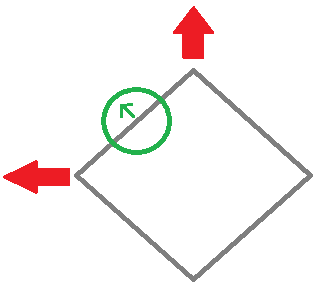
\includegraphics[scale=0.5]{Figures/ApertureProblem.png}
    \caption{Illustration of the Aperture problem. Moving the gray rectangle in the direction of any of the two red arrows both give the movement shown by the green arrow if seen through the green circled aperture.}
    \label{ApertureProblem}
\end{figure}



\section{The Smoothness Constraint}
As noted in the previous section, the system does not admit a unique solution with the constraints given so far. A common approach, an idea introduced by Horn and Schunck \cite{HS}, is to incorporate a smoothness constraint in the model. This smoothness constraint, also called the spatial coherence assumption \cite{Black199675}, says that points can not move independently in the brightness pattern. There has to be some smoothness in the flow vector for points belonging to the same object. In other words, points on the same object moves with the same velocity. A natural way of obtaining a smoother solution would be to minimize some term depending on the sizes of the gradients $\nabla u$ and $\nabla v$. As noted by Horn and Schunck, this leads to problems where one would expect discontinuous flow patterns. This is the case in images where occlusions are present, for instance an image of an object moving in a snow storm.

\section{Variational Formulation}
The aim now is to be able to combine these two constraint into one functional to be minimized. Now define
\begin{align*}
\Upsilon_0(\textbf{w}) = \nabla f \cdot \textbf{w} + f_t.
\end{align*}
If the constraint (\ref{BC}) coming from the brightness constancy assumption is to be satisfied, one would want to minimize a function that penalizes high values of $\Upsilon$. For now this term is called the data term $M(u,v)$. At the same time one would want to satisfy the smoothness constraint, that is, one would want to define a smoothness function that depends on the values of the gradients $\nabla u$ and $\nabla v$. Let this smoothness function be denoted as $V(\nabla u, \nabla v)$. To minimize both $M(u,v)$ and $V(\nabla u, \nabla v)$ one forms the following global energy function:
\begin{align}
\label{OF_funtional}
E(u,v) = \frac{1}{2} \int_\Omega (M(u,v) + \frac{1}{\sigma^2} V(\nabla u, \nabla v)) \, dx \, dy,
\end{align}
where $\sigma > 0$ is a regularization parameter. The problem is now to find the minimum of the energy functional $E(u,v)$. From calculus of variations we have that if $\textbf{w}$ minimizes a functional
\begin{align*}
J(\textbf{w}) = \iint \limits_\Omega F(x,y,\textbf{w},\textbf{w}_x,\textbf{w}_y) \, dx \, dy,
\end{align*} 
then the first variation must be zero,
\begin{align*}
\delta J(\textbf{w};\bm{\eta}) = \frac{d}{d \epsilon} \left[ J(\textbf{w} + \epsilon \bm{\eta}) \right] = 0,
\end{align*}
at $\epsilon = 0$ for any arbitrary function $\bm{\eta}(x,y)$. We get
\begin{align*}
\delta J(\textbf{w};\bm{\eta}) =&  \iint \limits_{\Omega} \frac{d}{d \epsilon}\Big|_{\epsilon = 0} F(x,y,\textbf{w} + \epsilon \bm{\eta}, \textbf{w}_x + \epsilon \bm{\eta}_x, \textbf{w}_y + \epsilon \bm{\eta}_y) \, dx \, dy \\
=&  \iint \limits_{\Omega} \bm{\eta} F_\textbf{w} + \bm{\eta}_x F_{\textbf{w}_x} + \bm{\eta}_y F_{\textbf{w}_y} \, dx \, dy \\
=& \iint \limits_{\Omega} \bm{\eta} F_\textbf{w} + \frac{d}{d x} (\bm{\eta} F_{\textbf{w}_x}) + \frac{d }{d y} (\bm{\eta} F_{\textbf{w}_y}) - \bm{\eta} \left( \frac{d}{d x} F_{\textbf{w}_x} + \frac{d }{d y} F_{\textbf{w}_y} \right) \, dx \, dy.
\end{align*}
Now let $\Gamma_{E}$, $\Gamma_{W}$, $\Gamma_{N}$ and $\Gamma_{S}$ be the east, west, north and south boundary of our domain respectively. Then using Gauss' Theorem gives
\begin{align*}
& \iint \limits_{\Omega}  \frac{d}{d x} (\bm{\eta} F_{\textbf{w}_x}) + \frac{d }{d y} (\bm{\eta} F_{\textbf{w}_y}) \, dx \, dy \\ 
=  &\int_{\Gamma_{E}} \bm{\eta} F_{\textbf{w}_x} \, dx - \int_{\Gamma_{W}} \bm{\eta} F_{\textbf{w}_x} \, dx + \int_{\Gamma_{N}} \bm{\eta} F_{\textbf{w}_y} \, dy - \int_{\Gamma_{S}} \bm{\eta} F_{\textbf{w}_y} \, dy
\end{align*}
Using this result, we get
\begin{multline*}
\delta J(\textbf{w};\bm{\eta}) = \iint \limits_{\Omega} \bm{\eta} \left( F_\textbf{w} -  \frac{d}{d x} F_{\textbf{w}_x} - \frac{d }{d y} F_{\textbf{w}_y} \right) \, dx \, dy  \\ 
+  \left( \int_{\Gamma_{E}} \bm{\eta} F_{\textbf{w}_x} \, dx - \int_{\Gamma_{W}} \bm{\eta} F_{\textbf{w}_x} \, dx + \int_{\Gamma_{N}} \bm{\eta} F_{\textbf{w}_y} \, dy - \int_{\Gamma_{S}} \bm{\eta} F_{\textbf{w}_y} \, dy \right) = 0.
\end{multline*}
Since this must hold for any arbitrary function $\bm{\eta}(x,y)$ it follows that
\begin{align*}
F_{\textbf{w}} - \frac{d}{dx} F_{\textbf{w}_x} - \frac{d }{d y} F_{\textbf{w}_y} &= 0 \quad \text{in} \ \Omega \\
F_{\textbf{w}_x} &= 0 \quad \text{on} \ \Gamma_e \ \text{and} \ \Gamma_w \\
F_{\textbf{w}_y}& = 0 \quad \text{on} \ \Gamma_n \ \text{and} \ \Gamma_s
\end{align*}
This is called the Euler-Lagrange equation of variational calculus. From this result it is easy to see that the following must hold for (\ref{OF_funtional}):
\begin{equation}
\label{EL}
  \begin{aligned}
\partial_{\textbf{w}} M - \frac{1}{\sigma^2}\left( \frac{d}{d x} \partial_{\textbf{w}_x} V + \frac{d}{d y} \partial_{\textbf{w}_y} V \right) &= 0 \quad \text{in} \ \Omega,  \\
\partial_{\textbf{w}_x} V &= 0 \quad \text{on} \ \Gamma_E \ \text{and} \ \Gamma_W, \\
\partial_{\textbf{w}_y} V &= 0 \quad \text{on} \ \Gamma_N \ \text{and} \ \Gamma_S.
  \end{aligned}
\end{equation}

\section{Penalizing The Data Term}
\label{sec:Data_penalization}
When the brightness constancy assumption was first introduced, Horn and Schunck used a quadratic penalization of $\Upsilon$,which is equivalent to least-squares minimization, but other penalization functions have been proposed. Least-squares minimization is very sensitive to outliers. In the case of the data term, these outliers would be noise in the image (a pixel that jumps from low intensity to high intensity without corresponding to the motion of an object). Black and Anandan \cite{Black199675} proposed several subquadratic penalizer functions, arguing that a subquadratic penalizer would improve the robustness in the presence of outliers. In general the data term $M(u,v)$ can be written as
\begin{align}
\label{DataPenalize}
M(u,v) = \Psi_M(\Upsilon_0^2),
\end{align}
where $\Psi_M(s^2)$ is some penalizing function aiming to minimize $\Upsilon_0^2$. 

\section{Penalizing The Smoothness Term}
The smoothness terms considered here will be quadratically dependent on the gradient in each direction, thus it is convenient to write the smoothness term in the form
\begin{align}
\label{SmoothnessTerm}
V(\nabla u, \nabla v) = \Psi_V(\nabla u ^T \Theta_u \nabla u) + \Psi_V(\nabla v ^T \Theta_v \nabla v),
\end{align}
where $\Psi_V(s^2)$ is a penalizing function that can be either quadratic or subquadratic, and $\Theta_u = \Theta_u(x,y,u,v)$ and $\Theta_v = \Theta_v(x,y,u,v)$ are matrices steering the diffusion process of the Euler-Lagrange system (\ref{EL}). Their eigenvectors and corresponding eigenvalues gives the direction and magnitude of smoothing respectively.

\section{The Euler-Lagrange System}
After defining the data term and the smoothness term using penalizing functions one can see that equation (\ref{EL}) takes the form
\begin{equation}
\label{EL_regu}
\begin{aligned}
\Psi_M'(\Upsilon_0^2)(f_xu+f_yv + f_t)f_x - \frac{1}{\sigma^2} \text{div} \left(\Psi_V'(\nabla u^T \Theta_u \nabla u)  \Theta_u \nabla u \right) = 0 \\
\Psi_M'(\Upsilon_0^2)(f_xu+f_yv + f_t)f_y - \frac{1}{\sigma^2} \text{div} \left(\Psi_V'(\nabla v^T \Theta_v \nabla v)  \Theta_v \nabla v \right) = 0
\end{aligned}
\end{equation}
for $(x,y) \in \Omega$ with Neumann boundary conditions. The theoretical framework presented up to this point is the same for all the methods considered here. The main distinction for each method will be across which boundaries the flow field is smoothed, that is, the choice of diffusion matrix. We start with the simplest choice; the uniform smoothness approach by Horn and Schunck.
